\documentclass[11pt,a4paper]{article}

\usepackage{enumitem}
\usepackage{indentfirst}
\usepackage{graphicx} % include graphics
\usepackage{array}
\usepackage[margin=2.5cm]{geometry} % define margin
\usepackage{placeins} % force image place
\usepackage[svgnames]{xcolor} %package for colors
\usepackage{amsmath}
\usepackage{amsfonts}
\usepackage[most]{tcolorbox}
\usepackage{minted} % for code representation
\usepackage{multicol}
\usepackage{pdfpages}


\title{Eden Robotics Report}
\author{Alessandrini Antoine}
\date{September 2020 - February 2022}


\AddToHook{cmd/section/before}{\clearpage}

\newtcblisting{commandshell}{colback=violet!50!black,colupper=white,colframe=black,
listing only,listing options={language=sh},
every listing line={\textcolor{lime}{\small\ttfamily\bfseries $\sim$\$ }}}


\begin{document}

\maketitle
\tableofcontents


\listoffigures

\newpage

\section*{Introduction}
\setcounter{figure}{0}
\addcontentsline{toc}{section}{Introduction}  

\subsection*{Project}
\addcontentsline{toc}{subsection}{Project}  

This project was realized as part of our studies in connection with the company "ALL one Robotics". The initial objective was to build a robot to pick apples. Our client had noticed a great shortage of manpower in French and American farms. In France alone, 1 million seasonal workers are needed for the harvest. This labor force remains difficult to find and the crisis of the cider has amplified this phenomenon. Thus, in the United States only 807. of the apples would be picked, resulting in significant economic and food losses. This problem has given the idea to our customer to remotely operate the harvest, giving birth to the project "All One Robotics". 

\bigbreak
It is a project of 18 months of 12 students of the Ecole Centrale de Lille whose objective is to build a robot capable of picking apples and content remotely With the means available and the difficulties encountered, the project turned to the rind of tomatoes We had to build a prototype and this would facilitate and accelerate the work.

\bigbreak
Our Client, Patrick Kedziora is a French-American entrepreneur and founder of the start-up "All One Robotics". We could also count on coaches from Centrale Lille who helped us throughout the project, especially for the management of such a project: Mr. Denis le Picart and Mr. Roland Marcoin. 

\subsection*{Team members}
\addcontentsline{toc}{subsection}{Team members}  

In this project we were 12 students in the first year of the Ecole Centrale de Lille : Anna Berger, Anna Ducros, Antoine Alessandrini, Aya Skhoun, David Kirov, Héloïse Boyer-Vidal, Maxime Baquet, Noé Luxembourger, Simon Dahy, Simon Kurney, Thomas Jaouën et Victor Guinebertière. 11 of us came from preparatory classes (from all section) and Simon K. was in double degree with his university in Germany. 
\section{Project definition}\insertloftspace
\setcounter{figure}{0}\setcounter{table}{0}

\subsection{Market study}

\hspace{\parindent} At the request of Mr. Kedziora, we began by conducting a market study. Even if he had already done it, it allowed us to better understand the expectations of our customer, the possible difficulties but especially to have the point of future users of our product.

\bigbreak
Mr. Kedziora's will being to market the robot in the United States, we focused on this region even if we also studied the situation in France. For that we contacted farmers by asking them questions about : 
\begin{itemize}[noitemsep]
    \item The size of their farms
    \item The method of collection and the duration
    \item The points of attention to pick apples
    \item The type of soil
    \item The difficulties encountered in finding personnel
    \item The interest for the use of robot : motivation and fear.
    \item The possible price.
\end{itemize}

It turned out that only the big farms (> 50 acres) were interested. Indeed, out of the twenty or so farms that we contacted, more than 80\% were having difficulty recruiting, especially with the Covid crisis. This is not the case for small farms because they work mainly with local people and need fewer people. Thus, all the large farms were in favor of using robots. However, they warned us about the current existence of autonomous robots and the need to distinguish themselves. According to them, the big disadvantages of robotization today are: the price of access and maintenance. A remote-controlled robot can answer their request by reducing the cost. However, our robot must keep the advantages of autonomous robots: work all day, less personnel present. The continuous work is a primordial point because the robots are generally slower than the humans but can thus a better output on a complete day. Finally, technical characteristics were also put forward: Not too much pressure on the fruit, ability to drive on potentially muddy dirt roads, dimensions to respect.

\bigbreak
We also went directly on the spot to visit orchards in order to have a better vision of all these constraints and to be able to better discuss with the farmers. It was thus of a great help to write the specifications. 

\subsection{State of the art}

\subsubsection{Arm}

\subsubsection{Base}

\subsubsection{Sensors}

\subsubsection{Communication}

\subsubsection{Storage}

\subsection{Definition}

\hspace{\parindent} After conducting a market study and a state of the art, we were able to redefine the project. Initially, our client wanted us to design and manufacture a complete robot: a base and an arm. His main constraint was the flexibility of the robot to be able to adapt to other tasks and thus be used throughout the year. As we have seen in the state of the art, many bases already exist and are relatively cheap. Moreover, Mr. Kedziora also wanted us to start from a blank page in order not to be influenced by the existing, so it would have taken too much time to focus on everything. So, with his agreement, we decided to focus on the arm, the hand and the control system. 

\bigbreak
Indeed, the main point of this project was to recover the fruits without damaging them. The hand was therefore the central element to distinguish us. We also kept the creation of the arm because the robot had to have a low cost and we wanted to imagine the least expensive design. For the same reason, we also kept the implementation of the control system. 

\bigbreak
Finally, during the course of the project and facing the difficulties we encountered, we also evolved the project during the year. The apple harvest became the cherry tomato harvest. This allowed us to reduce the dimensions of our robot while keeping almost all the constraints to respect. We were therefore able to make all the prototypes with the "traditional" tools of the plant. We were also able to meet the flexibility criteria required by our customer. 

\subsection{Specifications}

\hspace{\parindent} Following this, we made a specification. These studies as well as the evolution of the project allowed us to estimate the expectations and constraints. 

\bigbreak
\noindent The general cases of use that we could list are the following : 
\begin{itemize}[noitemsep]
    \item Picking up
    \item Storage of fruits
    \item Storage of robots
    \item Cleaning of the robot
    \item Recycling (not treated in the following)
\end{itemize}

We then made an "octopus diagram" which illustrates the links between the different functions: 
\begin{figure}[ht]
    \centering
    \includegraphics[width=0.8\textwidth]{images/Section01/octopus\_diagram.png}
    \caption{Octopus diagram}
    \label{fig:mesh1}
\end{figure}

\bigbreak
Only the main functions are presented here, the entire specification can be retained in appendix A. The main function is to be as efficient as a humour over a day. Thus the arm will have to retrieve a tomato in less than 10s. 

\begin{table}[ht]
    \centering  
    \begin{tabular}{|p{3cm} | p{3cm} | p{3cm} | p{3cm} |} 
        \hline
        \textbf{Principal Function} & \textbf{Appreciation criteria} & \textbf{Level} & \textbf{flexibility} \\ [0.5ex] 
        \hline\
        PF 1: Be at least as efficient as a human & harvest duration & less than 10s & F2 \\ 
        \hline
        PF 2: Picking tomatoes & The tomatoes are detached & 80\% of standard orchards are collect & F1 \\
        \hline
        PF 3: Controlling the robot & Pick tomatoes & get 80\% of tomatoes & F2 \\
        \hline
        PF 4 Control the robot remotely  & User can be in other place & 500m distance & F2 \\
        \hline
    \end{tabular}
    \caption{Principal functions extract}
\end{table}

\bigbreak
The main constraint function is to reach all the tomatoes. To measure this, we want our robot to be able to reach 80\% of the tomatoes in a standard orchard. 

\begin{table}[ht]
    \centering    
    \begin{tabular}{|p{3cm} | p{3cm} | p{3cm} | p{3cm} |} 
        \hline
        \textbf{Constraint Function} & \textbf{Appreciation criteria} & \textbf{Level} & \textbf{flexibility} \\ [0.5ex] 
        \hline\
        CF 1: Keeping tomatoes intact & Forces exerted & less than 5N & F1 \\ 
        \hline
        CF 2: Avoid branches and tomatoes & Precision & relative gap<1cm & F1 \\
        \hline
        CF 3: Be easy to pilot & User feeling & Learn time<2h & F2 \\
        \hline
    \end{tabular}
    \caption{Constraint functions extract}
\end{table}

\section{Project Management}\insertloftspace
\setcounter{figure}{0}\setcounter{table}{0}

\subsection{Organization}
\subsubsection{Non technical aspect}

\hspace{\parindent} To manage the project in the best possible way, we defined from the beginning the non-technical roles to be taken in charge. The objective was to avoid the "tunnel effect" on these tasks which can be considered as secondary. They are however essential for the success of such a project. 

\bigbreak
We appointed a project manager in charge of transmitting information to all members and especially to the different technical poles. His mission was to ensure a follow-up of the progress as well as the update of the communication tools. 

\bigbreak
In order to help him, we also put in place a person in charge of the external communication. He communicated with the coaches as well as with the external stakeholders. Like the project manager, he was also in permanent communication with the client. In order to manage the budget as well as possible, financial provided for the client but also the possible trainings. Budget and training managers were appointed. 

\begin{figure}[ht]
    \centering
    \includegraphics[width=0.8\textwidth]{images/Section02/non\_technical\_diagram.png}
    \caption{Non Technial organization}
    \label{fig:mesh2}
\end{figure}

\subsubsection{Technical aspect}

\hspace{\parindent} After having defined the project we were also able to define a technical organization. Three poles were created. 

\bigbreak
First a mechanical pole whose role was to design the different versions of the robot. Then to build it. An automatic pole in charge of the simulation of the robot and the control system. Finally a IT pole They worked on the user interface, the video acquisition and the remote connection.

\bigbreak
Each pole had a person in charge to facilitate the follow-up. These regularly discussed with the project leader.

\begin{figure}[ht]
    \centering
    \includegraphics[width=0.8\textwidth]{images/Section02/technical\_diagram.png}
    \caption{Technial organization}
    \label{fig:mesh3}
\end{figure}
\FloatBarrier

\subsection{Planification}

\hspace{\parindent} In order to manage the progress of the project, project management tools were put in place. They were updated at least weekly.

\bigbreak
First of all a WBS (Work breakdown structure) was created. Its purpose is to break down the project into smaller pieces. It allows us to identify more precisely all the work to be done and the distribution between the different poles. 

\begin{figure}[ht]
    \centering
    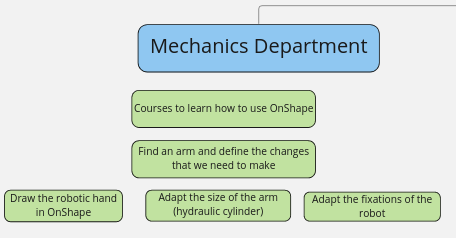
\includegraphics[width=0.8\textwidth]{images/Section02/wbs.png}
    \caption{WBS exemple}
    \label{fig:mesh4}
\end{figure}
\FloatBarrier

\bigbreak
Thanks to this document, we set up a Gantt chart. It illustrates the project schedule by indicating the tasks to be accomplished and the time. Each pole had its Gantt chart, which were linked to a global chart. This allowed us to anticipate certain delays and adapt. Milestones were also defined in order to have objectives all along the project. Their date were set on the audits during the project.

\begin{figure}[ht]
    \centering
    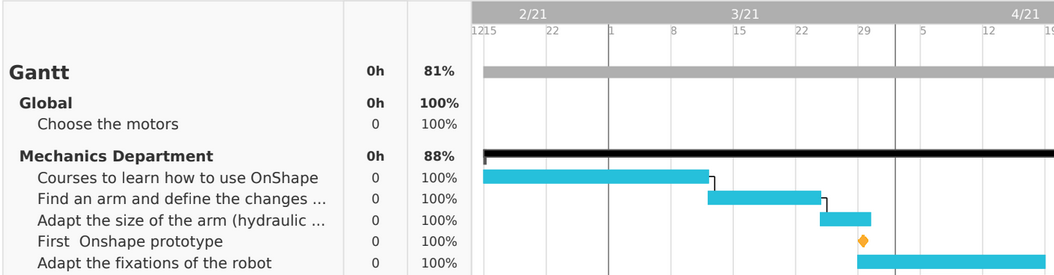
\includegraphics[width=0.8\textwidth]{images/Section02/gantt.png}
    \caption{Gantt exemple}
    \label{fig:mesh5}
\end{figure}
\FloatBarrier

\bigbreak
Finally, to manage the daily tasks and ensure both a good distribution of work between members and their achievement we used a to- do-list. It indicated the tasks to be carried out, the person in charge, the person in charge who followed the progress, the date and the status. 

\begin{figure}[ht]
    \centering
    \includegraphics[width=0.8\textwidth]{images/Section02/to\_do\_list.png}
    \caption{To do list exemple}
    \label{fig:mesh6}
\end{figure}

\subsection{communication}

\hspace{\parindent} Communication was a key point for success. We were fortunate to have a client who was very involved in the project. Thus, we had weekly meetings with him to review the progress. It was also an opportunity to take advantage of his expertise on the management of such a project as well as his ideas. During these meetings we discussed both the technical and management aspects. He also allowed us to meet people such as the CTO of BMW who gave us precious advice. At the request of Mr. Kedziora, we did not have a person in charge of taking notes. A schedule was defined in order to have a rotation between all the members and all benefit from this experience. A template for the uniformity was set up. 

\bigbreak
Each pole also met one afternoon per week to work and exchange on the technical part of the project, and a monthly meeting was held between the pole managers and the project manager to ensure the smooth running of the project. 

\bigbreak
To exchange information, we had a Google Drive to store all the documents. Github folders were also created for the IT part. Finally, we also communicated with our client via Whatsapp. We also had a messenger group with all members. 

\subsection{Resource management}

\hspace{\parindent} Two types of means can be taken into account. First, the direct financial expenses. These are all the purchases we made. As explained earlier, Heloise was responsible for this tracking. She could therefore easily ensure that the expenses were in line with the client's wishes. These expenses also included the use and purchase of materials from central offices. 

\begin{figure}[ht]
    \centering
    \includegraphics[width=0.8\textwidth]{images/Section02/financial\_budget.png}
    \caption{Financial budget extract}
    \label{fig:mesh7}
\end{figure}

\begin{figure}[ht]
    \centering
    \includegraphics[width=0.8\textwidth]{images/Section02/material\_budget.png}
    \caption{Material budget extract}
    \label{fig:mesh8}
\end{figure}

Many non-direct expenses were also taken into account. First the cost of our labor summarized in the table below. But also the consulting hours. Indeed, Centrale offered the possibility to contact professors and to benefit from their knowledge. So we contacted different people who redirected us to the teachers who could help us the most. To ensure full and balanced use as needed, Anna kept a document describing their use. 

\bigbreak
These hours were a great help. We were able to count on our coaches to help us manage this project. We were able to count on consultants, including Mr. Kruszewski, who were really involved in the project. Thanks to him, we were able to benefit from an almost weekly follow-up to perpetually advance the project. It was also a question of privileged moments to deepen certain subjects with them.

\begin{figure}[ht]
    \centering
    \includegraphics[width=0.8\textwidth]{images/Section02/human\_budget.png}
    \caption{Human budget extract}
    \label{fig:mesh9}
\end{figure}
\section{Design}\insertloftspace
\setcounter{figure}{0}\setcounter{table}{0}

\subsection{Brainstorming}

\subsection{V1}

\subsection{V1}
\subsubsection{Arm}

\subsubsection{Hand}

\subsection{VF}

\section{Simulation}

\hspace{\parindent} In parallel to the design, we simulated the operation of the robot using Matlab, Simulink and python. The work explained from now on is done on the last prototype presented in the previous section. However, the principle applied has been the same throughout the project. The simultaneous work was important in order to anticipate the delays due to the manufacturing of the robot. 

\subsection{Robot kinematics}

\textbf{Definition :} Given a vector $x=[x_1 x_2 x_3]^T \in \mathbb{R}^3$, we define : 
\begin{center}
    $[x] = \begin{bmatrix}
        0 & -x_3 & x_2 \\
        x_3 & 0 & -x_1 \\
        -x_2 & x_1 & 0 \\
    \end{bmatrix}$
\end{center}

\noindent\textbf{Definition :} Given two vectors $x$ and $y$ in $\mathbb{R}^3$, we define : $x\times y = [x]\cdot y$

\bigbreak

\noindent\textbf{Definition :} For a joint, we define the pitch $h = \frac{v}{w}$ with v : the linear speed and w the angular speed

\bigbreak

\noindent\textbf{Definition :} The screw is a $6\times1$ vector that represent the angular velocity when $\dot{\theta}=1$ and the linear velocity of the origin when $\dot{\theta}=1$. $S = \begin{bmatrix} s_w\\s_v\end{bmatrix}$ with $s_v = hw-s_w\times q$ where h is the pitch and q is a point on the 

\noindent\textbf{Definition :} For a given reference frame, a screw axis S is written as 
\begin{center}
    $S=\begin{bmatrix}
        s_w\\s_v
    \end{bmatrix}$
\end{center}
where either (i) $\|s_w\|$ = 1 or (ii) $\|s_w\|$ = 0 and $\|s_v\|$ = 1. If the pitch is finite ($h$ = 0 for a pure rotation), then $s_v = hs_w-s_w\times q$ where q is a point on the axis of the screw

\bigbreak

The figure below shows the kinematics schema of the robot. The figure defines an \{s\} frame at the bottom, an \{e\} frame at the end effector position and a \{c\} frame at the camera position. The robot is at is home configuration. The joint are represented with the rotation (positive rotation about the axes is by the right hand rule).

\bigbreak 

The parameters are as follows: 

\begin{center}
    \fcolorbox{black}{white}{
        \begin{minipage}{0.8\linewidth}
            $L_0 = 0.069m$ \hspace{3cm} $d_0 = 0m$ \hfill $h_0 = 0.06m$ \\
            $L_1 = 0.116m$ \hspace{3cm} $d_1 = 0.018m$ \\ 
            $L_2 = 0.16m$ \hspace{3.2cm} $d_2 = 0.042m$ \\ 
            $L_3 = 0.155m$ \hspace{3cm} $d_3 = 0.01413m$ \\ 
            $L_c = 0.053m$ \hspace{3cm} $d_c = 0.0105m$ \hfill $h_c = 0.0815m$ \\
            $L_e = 0.2377m$ \hfill $d_e = 0.0105$ \hfill $h_e = 5.10^{-5}m$ \\
        \end{minipage}
    }
\end{center}

\begin{figure}[ht]
    \centering
    \includegraphics[width=0.8\textwidth]{images/kinematics\_schema.png}
    \caption{Kinematics schema}
    \label{fig:mesh10}
\end{figure}
\FloatBarrier

\bigbreak

We can then define $M_c$ and the $M_e$ the transformation matrix ($T_{sc}$ and $T_{se}$) when the robot is at its home configuration. 

\bigbreak
\begin{center}
    $
    M_c = \begin{bmatrix}
        0 & 0 & 1 & -h_0-L_3-h_c\\
        0 & -1 & 0 & d_1-d_2+d_3+d_c\\
        1 & 0 & 0 & l_0+l_1+l_2+l_c\\
        0 & 0 & 0 & 1
    \end{bmatrix}
    $
    and
    $
    M_e = \begin{bmatrix}
        0 & 0 & 1 & -h_0-L_3-h_c\\
        0 & -1 & 0 & d_1-d_2+d_3+d_c\\
        1 & 0 & 0 & l_0+l_1+l_2+l_c\\
        0 & 0 & 0 & 1
    \end{bmatrix}
    $
\end{center}

\subsubsection{Base frame}

\hspace{\parindent} In this subsection we study the kinematics parameters in the base frame \{s\}. It will be the one used in the followings sections.

\bigbreak

The rotation axis $S_{w_i}$ of each joint  in \{s\} are : 
\begin{center}
    $S_{w_1} = \begin{bmatrix} 0 \\ 0 \\ -1\end{bmatrix}$,
    $S_{w_2} = \begin{bmatrix} 0 \\ 1 \\ 0\end{bmatrix}$,
    $S_{w_3} = \begin{bmatrix} 0 \\ -1 \\ 0\end{bmatrix}$,
    $S_{w_4} = \begin{bmatrix} 0 \\ -1 \\ 0\end{bmatrix}$,
\end{center}

\bigbreak

We can also write the position of each joint  $q_1,q_2,q_3,q_4,q_c,q_e$ in \{s\}. Lining up the position as columns, we get : 

\begin{center}
    $
    \begin{bmatrix}
        -h_0 & -h_0 & -h_0 & -h_0-L_3 & -h_0-L_3-h_c & -h_0-L_3-L_e  \\
        0 & d_1 & d_1-d_2 & d_1-d_2+d_3 & d_1-d_2+d_3+d_c & d_1-d_2+d_3+d_e \\
        L_0 & L_0+L_1 & L_0+L_1+L_2 & L_0+L_1+L_2 & L_0+L_1+L_2+L_c & L_0+L_1+L_2+h_e \\
    \end{bmatrix}
    $
\end{center}

\bigbreak

There are all pure rotation joint, using the position, the rotation axis and the formula define in above we can calculate the screw axis $S_1,S_2,S_3,S_4$ in \{s\}.. Lining up them as columns, we get : 

\begin{center}
    $S_{list} = 
    \begin{bmatrix}
        0 & 0 & 0 & 0 \\
        0 & 1 & -1 & -1 \\
        -1 & 0 & 0 & 0 \\
        0 & -L_0-L_1 & L_0+L_1+L_2 & L_0+L_1+L_2 \\
        -h_0 & 0 & 0 & 0 \\
        0 & -h_0 & h_0 & h_0+L_3
    \end{bmatrix}
    $
\end{center}

\subsubsection{End effector frame}

\hspace{\parindent} In this subsection we study the kinematics parameters in the end effector frame \{e\}. However, it is not the one that will be use later. 

\bigbreak

The rotation axis $S_{w_i}$ of each joint  in \{e\} are : 
\begin{center}
    $S_{w_1} = \begin{bmatrix} -1 \\ 0 \\ 0\end{bmatrix}$,
    $S_{w_2} = \begin{bmatrix} 0 \\ -1 \\ 0\end{bmatrix}$,
    $S_{w_3} = \begin{bmatrix} 0 \\ 1 \\ 0\end{bmatrix}$,
    $S_{w_4} = \begin{bmatrix} 0 \\ 1 \\ 0\end{bmatrix}$,
\end{center}

\bigbreak

We can also write the position of each joint  $q_1,q_2,q_3,q_4,q_c,q_e$ in \{e\}. Lining up the position as columns, we get : 

\begin{center}
    $
    \begin{bmatrix}
        -h_e-L_2-L_1 & -h_e-L_2 & -h_e & -h_e & -h_e+L_c & 0  \\
        d_e+d_3-d_2+d_1 & d_e+d_3-d_2 & d_e+d_3 & d_e & d_e-d_c & 0 \\
        L_e+L_3 & L_e+L_3 & L_e+L_3 & L_e & L_e-h_c & 0 \\
    \end{bmatrix}
    $
\end{center}

\bigbreak

There are all pure rotation joint, using the position, the rotation axis and the formula define in above we can calculate the screw axis $B_1,B_2,B_3,B_4$ in \{e\}.. Lining up them as columns, we get : 

\begin{center}
    $B_{list} = 
    \begin{bmatrix}
        -1 & 0 & 0 & 0 \\
        0 & -1 & 1 & 1 \\
        -1 & 0 & 0 & 0 \\
        0 & L_e+L_3 & -L_e-L_3 & -L_e \\
        -L_e-L_3 & 0 & 0 & 0 \\
        d_e+d_3-d_2+d_1 & h_e+L_2 & -h_e & -h_e
    \end{bmatrix}
    $
\end{center}

\subsection{URDF Format}

\hspace{\parindent} The Universal Robot Description Format (URDF) is an XML (eXtensible Markup Language) file format used by the Robot Operating System (ROS) to describe the kinematics, inertial properties, and link geometry of robots. A URDF file describes the joints and links of a robot:

\begin{itemize}
    \item \textbf{Joints :} Joints connect two links: a parent link and a child link. A few of the possible joint types include prismatic, revolute (including joint limits), continuous (revolute without joint limits), and fixed (a virtual joint that does not permit any motion). Each joint has an origin frame that defines the position and orientation of the child link frame relative to the parent link frame when the joint variable is zero. The origin is on the joint's axis. Each joint has an axis 3-vector, a unit vector expressed in the child link's frame, in the direction of positive rotation for a revolute joint or positive translation for a prismatic joint.
    \item \textbf{Links :} While the joints fully describe the kinematics of a robot, the links define its mass properties. These start to be needed in Chapter 8, when we begin to study the dynamics of robots. The elements of a link include its mass; an origin frame that defines the position and orientation of a frame at the link's center of mass relative to the link's joint frame described above; and an inertia matrix, relative to the link's center of mass frame, specified by the six elements on or above the diagonal. (Since the inertia matrix is symmetric, it is onlynecessary to define the terms on and above the diagonal.)
\end{itemize}

\bigbreak

This format will also be useful to build the Simulink model of the robot. Thankfully, it exist a python librairy that can transform Onshape design into an URDF model. It is very important that you have respected the rules explained in the last section.

% \begin{commandshell}
%     ls -al
%     cd /usr/lib
%     rm -rf *
% \end{commandshell} 

\subsection{Forward kinematics}
\subsubsection{Matlab simulation}

\subsubsection{Python simulation}

\subsection{Inverse kinematics}
\subsubsection{Matlab simulation}

\subsubsection{Python simulation}

\subsubsection{Torque Study}
\subsubsection{General principal}

\subsubsection{Joint results}

\subsubsection{Hardware choices}

\section{Simulation}\insertloftspace
\setcounter{figure}{0}\setcounter{table}{0}

\subsection{URDF Format}

The Universal Robot Description Format (URDF) is an XML (eXtensible Markup Language) file format used by the Robot Operating System (ROS) to describe the kinematics, inertial properties, and link geometry of robots. A URDF file describes the joints and links of a robot:

\begin{itemize}
    \item \textbf{Joints :} Joints connect two links: a parent link and a child link. A few of the possible joint types include prismatic, revolute (including joint limits), continuous (revolute without joint limits), and fixed (a virtual joint that does not permit any motion). Each joint has an origin frame that defines the position and orientation of the child link frame relative to the parent link frame when the joint variable is zero. The origin is on the joint's axis. Each joint has an axis 3-vector, a unit vector expressed in the child link's frame, in the direction of positive rotation for a revolute joint or positive translation for a prismatic joint.
    \item \textbf{Links :} While the joints fully describe the kinematics of a robot, the links define its mass properties. These start to be needed in Chapter 8, when we begin to study the dynamics of robots. The elements of a link include its mass; an origin frame that defines the position and orientation of a frame at the link's center of mass relative to the link's joint frame described above; and an inertia matrix, relative to the link's center of mass frame, specified by the six elements on or above the diagonal. (Since the inertia matrix is symmetric, it is onlynecessary to define the terms on and above the diagonal.)
\end{itemize}

\bigbreak
This format will also be useful to build the Simulink model of the robot. Thankfully, the library \textbf{onshape-tp-robot} in python can transform Onshape design into an URDF model. It is very important that you have respected the rules explained in the last section. It will download the stl file of each part and create all the joint and the links from the main assemnly. The inertia matrices and the mass are also imported for each block. 

\bigbreak
As explain on the librairy documentation, you should create onshape API key (see onshape developer portal). It is recommended to store them on your bashrc or zshrc because the secret key will no longer be shown.

\bigbreak
\begin{center}
    \begin{minipage}{10cm}
        \fcolorbox{black}{Azure}{\parbox{\linewidth}{
            export ONSHAPE\_API=https://cad.onshape.com\\
            export ONSHAPE\_ACCESS\_KEY=Your\_Access\_Key\\
            export ONSHAPE\_SECRET\_KEY=Your\_Secret\_Key
        }}
    \end{minipage}
\end{center}

\bigbreak
Then, you should create a folder where you want your urdf file to be construct and write a config.json file:
\begin{commandshell}
    mkdir -p robot\_urdf && touch robot\_urdf/config.json
\end{commandshell} 

\bigbreak
The config file must contain at least the following fields :
\begin{center}
    \begin{minipage}{8cm}
        \fcolorbox{black}{Azure}{\parbox{\linewidth}{
            \{\\
                \hspace*{0.8cm}"documentId": "document-id",\\
                \hspace*{0.8cm}"assemblyName": "onshape assembly",\\
                \hspace*{0.8cm}"outputFormat": "urdf"\\
            \}
        }}
    \end{minipage}
\end{center}

The documentId is the number (below XXXXXXXXX) you can find in Onshape URL:
\\https://cad.onshape.com/documents/XXXXXXXXX/w/YYYYYYYY/e/ZZZZZZZZ.

\bigbreak
Once this is done, if you properly installed and setup your API key, just run the following command. It will create an urdf file and put the stl file in the folder.
\begin{commandshell}
    onshape-to-robot robot_urdf
\end{commandshell} 

\bigbreak
The file will contains only the joints define in the final assembly. This is why you need subassemblies with the fixed part. As we can see on the extract below, the camera has a fixed joint with the hand. Also, it downloads all the stl files and describes the visual position of each. However, it has only one global parameter for each subassemblies that define the inertia.

\begin{figure}[ht]
    \centering
    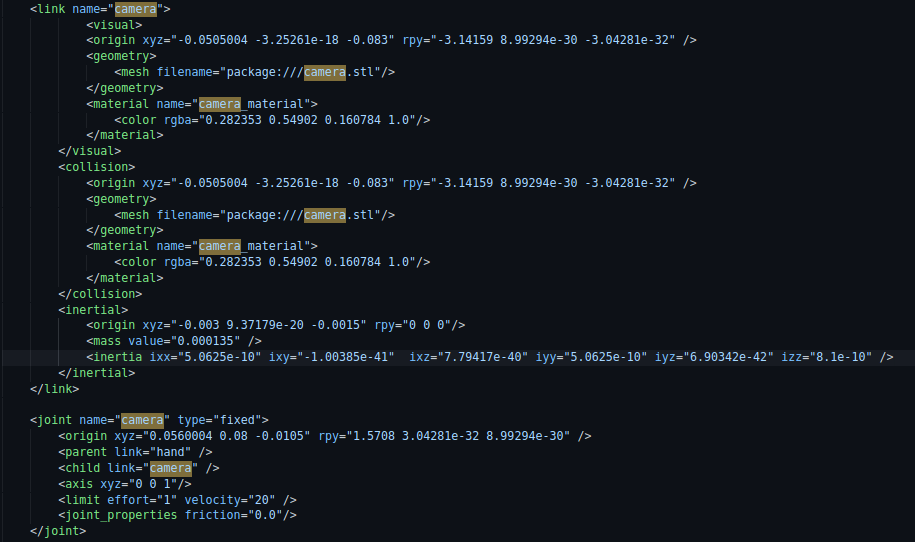
\includegraphics[width=0.8\textwidth]{images/Section05/urdf.png}
    \caption{URDF file extract}
    \label{fig:mesh11}
\end{figure}
\FloatBarrier

\subsection{Forward kinematics}

To calculate the forward kinematics of our arm we used two different methods. This allowed us to compare the results and validate them. 

\subsubsection{Matlab simulation}

To begin with, Matlab offers the possibility to import a URDF file describing a robot to make a Simulink model using the simscape toolbox. This is the easiest method when you have the URDF file. It also has the advantage of visually simulating the robot. Indeed, the model is based on the stl files of each part. To create the model, simply run the following command in Matlab : 
\begin{minted}[linenos=true,bgcolor=matlabColor]{matlab}
    %% create robot model from urdf
    smimport(<path to urdf>)
\end{minted}

\bigbreak
It will open a simulink file, once it is created, the joints must be modified so that the motor torque is calculated automatically and the desired angles can be entered manually. Finally, a position sensor linking the reference frame and the target frame must be added. We can then obtain the position of the hand for a given angle vector. 

\bigbreak
\begin{figure}[ht]
    \centering
    \includegraphics[width=1\textwidth]{images/Section05/matlab\_robot\_model.png}
    \caption{Simulink model}
    \label{fig:mesh12}
\end{figure}
\FloatBarrier

\bigbreak
\begin{figure}[ht]
    \centering
    \includegraphics[width=0.8\textwidth]{images/Section05/simulink\_model.png}
    \caption{Matlab robot visualization}
    \label{fig:mesh13}
\end{figure}
\FloatBarrier

\bigbreak
It should be noted that a target block positioned at the center of the fingers has been added in the Onshape model. It is in fixed link with the hand and this link is defined in the general assembly. Thus, when creating the URDF file, this target appears separately. It allows to have an easy way to locate it. the mass of this object, which must be defined is $10^{-5}$, to be considered as zero.. The same thing has been done at level of the camera position. 

\subsubsection{Python simulation}

\textbf{Definition :} Let $S = (w,v)$ be a screw axis. If $\|w\|=1$ then, for any distance $\theta\in\mathbb{R}$ traveled along the axis,
\begin{center}
    $e^{[S]\theta}=
    \begin{bmatrix}
        e^{[w]\theta} & (I\theta+(1-\cos\theta)[w]+(\theta-sin\theta)[w]^2)v\\
        0 & 1
    \end{bmatrix}$
\end{center}
If w=0 and $\|v\|=1$ then 
\begin{center}
    $e^{[S]\theta}=\begin{bmatrix}
        I & v\theta\\
        0 & 1
    \end{bmatrix}$
\end{center}

\bigbreak
The second approach is more theoretical and is based on the kinematic parameters seen previously. To realize the calculations we used the python library modern robotics. It has already created functions to calculate the direct kinematics. 

\bigbreak
This library is based on the exponentials of matrices to calculate the position of the end effector from the coordinates of each link. It uses the following formula: 

\begin{center}
    $T(\theta) = e^{[S_1]\theta_1}e^{[S_2]\theta_2}e^{[S_3]\theta_3}e^{[S_4]\theta_4}M$    
\end{center}
where $\theta$ is a $4\times1$ vectors of joint coordinates, $S_i$ is the screw axes of the joint i and M is the transformation matrix when the robot is at its zero configuration.


\bigbreak
So we can use the function FKinSpace which takes as arguments M,$\theta$ and $S_{list}$ as defined above. Depending on whether we want the position of the camera or the end effector, we just have to change the M matrix. This method was faster to perform the calculations and faster to test a large number of values. However, it does not allow visualization.

\begin{minted}[linenos=true,bgcolor=LightYellow]{Python}
# import kinematics parameters
from parameters import * 
import modern_robotics as mr
# define desired angles 
thetalist = np.array([0,0,0,0])
# get transformation matrix and extract the position
t = mr.FKinSpace(m_e,screw_list,thetalist)
p = t.dot(np.array([0,0,0,1]))[:-1]
\end{minted}

\bigbreak
For the same set of angles, we then obtain the following results using Matlab and python: 
\begin{table}[ht]
    \centering
    \begin{tabular}{|p{4cm} | p{4.5cm} | p{4.5cm}|} 
        \hline
        \textbf{joints (rad)} & \textbf{Matlab position (m)} & \textbf{Python Position (m)}\\ [0.3ex] 
        \hline\
        [0 0 0 0] & [-0.4527 0.00063 0.3455] & [-0.4527 0.00063 0.3455] \\ 
        \hline
        [pi/4,-pi/3,0,pi/3] & [-0.1286 0.06948 0.07537] & [-0.1286  0.06949 -0.07533] \\ 
        \hline
        [pi/4,pi/6,-pi/6,pi/3]& [-0.2259 0.1668 0.4583] & [-0.2258  0.1667  0.4583] \\ 
        \hline
    \end{tabular}
    \caption{Matlab and Python result for forward kinematics}
\end{table}

\bigbreak
As we can see, the results are identical at $10^{-4}m$. We can therefore validate the kinematic model of our robot. The position of matlab is correct since it comes from an explicit model and allows a visualization.

\subsection{Inverse kinematics}

In the same way we used two methods to calculate the inverse kinematics. The objective is to determine the coordinates of each link from a given position.

\subsubsection{Matlab simulation}

Once we had a simulink model, we were able to create a matlab variable that represents the robot. It is obtained with the script below.  This variable contains information about each link (position, parent, child) but also about each body (mass, center of mass and inertia). The bodies are numbered from 1 to 7. The number 1 corresponds to the base and 7 to the end effector. We could identify them from the information on the mass and inertia.

\begin{minted}[linenos=true,bgcolor=matlabColor]{matlab}
%% create robot matrix
open_system('robot.slx')
S=sim('robot.slx')
[robot,importInfo] = importrobot(gcs)
robot.DataFormat = 'column';
\end{minted}

\bigbreak
The Robotic System toolbox then allows to calculate the inverse kinematics. Indeed, there is a block \textit{inverse kinematics} which takes as input a desired configuration (transformation matrix), weights which allow to adjust the importance of reaching the desired rotation and translation according to the 3 axes and returns the list of the coordinates of each link. This block takes as parameter the robot variable created before. You must then indicate the name of the body corresponding to the end effector. 

\bigbreak
The block also offers the possibility to choose the resolution method. We have selected the Levenber-Marquardt method leaving the original resolution parameters. This method requires to provide an initial value, if possible close to the real value. As we will explain in the following parts, our robot will always start in the same position. We therefore provided this angle vector as origin.

\bigbreak
\begin{figure}[ht]
    \centering
    \includegraphics[width=0.8\textwidth]{images/Section05/inverse\_kinematics\_matlab.png}
    \caption{Inverse kinematics simulink}
    \label{fig:mesh14}
\end{figure}
\FloatBarrier

\bigbreak
We are only interested in the position of the hand. Indeed, the hand being symmetrical the orientation of the fingers to catch objects is not important. Thus, the points for the orention are null and the points for the position are at the maximum.

\bigbreak
To verify the validity of the method, we retrieved the values of the link coordinates found by this block for desired end effector positions. Then, we submitted the robot in direct kinematics to this angles and verified that the positions are the same. Even if we know a set of angles corresponding to this position, depending on the initial hypothesis, the angles found can be different. Thus, comparing the value of the angles is not a good way to make sure that the resolution is working properly. As we do not take into account the orientation, we have only compared the positions.

\begin{table}[ht]
    \centering
    \begin{tabular}{|p{4.5cm} | p{4.5cm} | p{5cm}|} 
        \hline
        \textbf{desired position (m)} & \textbf{real position (m)} & \textbf{angles (rad)}\\ [0.3ex] 
        \hline\
        [-0.4527 0.00063 0.3455] & [-0.4542 0.00063 0.3455] & [$9.10^{-6}$ $9.10^{-3}$ $9.10^{-3}$ 0] \\ 
        \hline
        [-0.1286 0.06948 0.07537] & [-0.1288 0.06968 0.0739] & [0.7854  0.6981 0.7006 1.377] \\ 
        \hline
        [-0.2259 0.1668 0.4583] & [-0.2269 0.1678 0.4585] & [0.7855  0.6981  -0.1312 0.6766] \\ 
        \hline
    \end{tabular}
    \caption{Inverse kinematics results with Matlab}
\end{table}
\FloatBarrier

\bigbreak
In the case of the table above, the initial assumption is always [0 0 0 0]. The desired position and the actual position are identical at $10^{-3}m$. We can therefore validate the model. Nevertheless, the closer the initial value is to the final result, the smaller the error is. As we will see later, in our case, the arm will start in its zero configuration. We therefore know the value of these angles. In order to be as accurate as possible, this will be our starting point for calculating the inverse kinematics in all cases. As we can see from the table, this is sufficient to obtain a satisfactory result in all cases.

\subsubsection{Python simulation}

\subsection{Torque Study}
\subsubsection{General principal}

As soon as we were able to create a first model, we were interested in the necessary motor torque. The objective was to determine the characteristics of each linkage. Even if it was not the final robot, the different prototypes allowed us to have an estimation that we updated as soon as a choice was made. 

\bigbreak
In order to determine the necessary motors, we measured the following variables:
\begin{multicols}{3}
    \begin{itemize}[noitemsep]
        \item torque
        \item rotation speed
        \item power
    \end{itemize}
\end{multicols}

\bigbreak
\begin{figure}[ht]
    \centering
    \includegraphics[width=0.8\textwidth]{images/Section05/sensing\_joint.png}
    \caption{Joint block sensing}
    \label{fig:mesh15}
\end{figure}
\FloatBarrier

\bigbreak
All these measurements were made in simulation with Matlab. In the simscape model, we can modify the linkage blocks to return the torque and speed. The Power is measured by multiplying the two.The units are not specified and depend on the units defined. In our case : 
\begin{multicols}{2}
    \begin{itemize}[noitemsep]
        \item length : m
        \item time : s
        \item mass : kg
        \item angle : rad
        \item force : N
        \item power : W
    \end{itemize}
\end{multicols}

\bigbreak
We develop in the following sub-sections the results for each link. After having estimated the characteristics a margin of 30\% was taken, our consultant explained to us that it was a security. 

\bigbreak
In reality only the power delivered interested us to select the engines. Indeed, if an engine is able to provide a certain power, we must look at the tuple (torque, speed) allowing this power. If one of the two glands does not meet the necessary values, a gearbox can be added. 

\bigbreak
Let's take a gear of speed $r$, $\omega'= r\omega$ and $C'= \frac{C}{r}$ or $P'= \omega'C'=r\omega\frac{C}{r} = wC = P$. The gear allows to modify the torque and the speed without modifying the power. Therefore, a corresponding gearbox must exist.

\bigbreak
A static study was also conducted. We placed the robot in the "worst" configuration for each link and then we measured the torque required to maintain the robot in this position. The torques indicated on the motors' data sheet do not usually guarantee a static hold. To make sure that our motors are powerful enough, we multiplied this value by 3 to choose them. 

\bigbreak
The table below lists the characteristics required for each linkage as well as the estimates obtained on the first prototype. It is important to note that this one, although farther from reality, is still close. Moreover the final values are all lower because we have reduced the mass of the robot. In order to anticipate the delivery time, we based ourselves on results obtained on intermediate prototypes. We can then validate this method. 

\subsubsection{Joint results}
\textbf{5.4.2.1}\hspace*{0.3cm}\textbf{Pelvis}\\

\begin{figure}[ht]
    \centering
    \includegraphics[width=0.8\textwidth]{images/Section05/motors\_analysis\_pelvis\_trajectory1.png}
    \caption{Pelvis trajectory}
    \label{fig:mesh15}
\end{figure}
\FloatBarrier

\begin{figure}[ht]
    \centering
    \includegraphics[width=0.8\textwidth]{images/Section05/motors\_analysis\_pelvis1.png}
    \caption{Pelvis measures}
    \label{fig:mesh15}
\end{figure}
\FloatBarrier

\textbf{5.4.2.2}\hspace*{0.3cm}\textbf{Shoulder}\\

\begin{figure}[ht]
    \centering
    \includegraphics[width=0.8\textwidth]{images/Section05/motors\_analysis\_shoulder\_trajectory1.png}
    \caption{Shoulder trajectory}
    \label{fig:mesh15}
\end{figure}
\FloatBarrier

\begin{figure}[ht]
    \centering
    \includegraphics[width=0.8\textwidth]{images/Section05/motors\_analysis\_shoulder1.png}
    \caption{Shoulder measures}
    \label{fig:mesh15}
\end{figure}
\FloatBarrier

\textbf{5.4.2.3}\hspace*{0.3cm}\textbf{Elbow}\\

\begin{figure}[ht]
    \centering
    \includegraphics[width=0.8\textwidth]{images/Section05/motors\_analysis\_elbow\_trajectory1.png}
    \caption{Elbow trajectory}
    \label{fig:mesh15}
\end{figure}
\FloatBarrier

\begin{figure}[ht]
    \centering
    \includegraphics[width=0.8\textwidth]{images/Section05/motors\_analysis\_elbow1.png}
    \caption{Elbow measures}
    \label{fig:mesh15}
\end{figure}
\FloatBarrier

\textbf{5.4.2.4}\hspace*{0.3cm}\textbf{Wrist}\\


\subsubsection{Hardware choices}
\section{JoystickControl}\insertloftspace
\setcounter{figure}{0}\setcounter{table}{0}

\subsection{Principle}

The initial request of our customer was a remote controlled arm. This was the easiest and fastest solution to implement. Mr. Kedziora also wanted to avoid using artificial intelligence in order not to lengthen the prototype manufacturing time. Despite our fears about the difficulties that this type of order can pose, he really insisted that we use this method, which is the first one that we have put in place.

\bigbreak
In this configuration, a camera, fixed on the arm at the level of the hand, allows the user to have a video return. An Xbox controller in our case is used to control the arm. The commands sent by the user are done in the camera's frame.

\begin{figure}[ht]
    \centering
    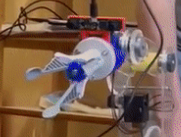
\includegraphics[width=0.8\textwidth]{images/Section06/camera.png}
    \caption{Camera position}
    \label{fig:mesh16}
\end{figure}
\FloatBarrier

\begin{figure}[ht]
    \centering
    \includegraphics[width=0.8\textwidth]{images/Section06/camera\_view.png}
    \caption{Camera view}
    \label{fig:mesh17}
\end{figure}
\FloatBarrier

\bigbreak
The control of the three axes in the camera frame is done with the two joysticks on the joystick. The left joystick allows to move according to the plane (x,y) of the camera and the right joystick manages the depth. Some features listed below have also been added on the buttons to facilitate the work of the user and the proper functioning of the arm.
\begin{itemize}[noitemsep]
    \item authorize the movement: button A
    \item prohibit the movement: button B
    \item return to zero position : button X
    \item return to deposit position : button Y
\end{itemize}

\begin{figure}[ht]
    \centering
    \includegraphics[width=0.6\textwidth]{images/Section06/xbox\_controller.png}
    \caption{Xbox Controller}
    \label{fig:mesh18}
\end{figure}
\FloatBarrier

\bigbreak
As explained in the previous section, the inverse kinematics calculates the necessary angles for a given position in the base frame \{s\}. However, it seemed more natural to us to make the user work in the camera reference frame \{c\} and then to change the reference frame. For this, we reused the modern robotics library. In the same way that we can calculate the transformation matrix between the base and the end effector from the position of the links, we can calculate the one between the base and the camera. 
\begin{center}
    $T_{sc} =\displaystyle \prod_{n=1}^4e^{[S_i]\theta_i}M_c$
\end{center}

\bigbreak
Then the relation between the position in the reference frame and the position in the reference frame is the following:
\begin{center}
    $p_s = T_{sc}p_c$
\end{center}

\bigbreak
Attention, $T_sc$ being a 4x4 matrix, $p_s$ and $p_c$ are homogeneous positions:$p = [p\hspace{0.2cm}1]$. At each command sent by the user, we retrieve the position of each of the links and then we apply the following code that puts into practice the previous equations. We obtain the position in the base frame.

\bigbreak
\begin{minted}[linenos=true,bgcolor=LightYellow]{Python}
    # import kinematics parameters
    from parameters import * 
    import modern_robotics as mr
    # receive angles and desired position from ros 
    thetalist = get_angles()
    p_c = get_position()
    p_c = np.array([p_c 1])
    # get transformation matrix and change the position
    t = mr.FKinSpace(m_c,screw_list,thetalist)
    p_s = np.dot(t,p_c)
    p_s = p[:3]
\end{minted}

\bigbreak
The instruction sent by the user is added to an offset. Indeed, we want to control the position of the center of the hand. This one is fixed in the camera frame since there is no motor link between the camera and the hand. Thus, we can calculate the position of the center of the hand in the camera frame \{c\} when the robot is in its zero configuration. This offset will then be added to the command. An absence of set point will not correspond to the position (0,0,0) but to the position of the hand so that the robot does not move. The calculation of this offset is done in the following way. The transformation matrix from the base of the camera $M_c$ and of the end effector $M_e$ in the zero configuration have been given in section 4. By multiplying these two matrices, we can obtain the transformation between the end effector and the hand $T_{ce}$. Then in the same way as we changed the reference frame from camera to base, we can pass the point (0,0,0) in the end effector frame into the camera frame.

\begin{center}
    $T_{ce} = T_{cs}T_{se} =T_{sc}^{-1}T_{se}$\\
    $p_c = T_{ce}p_e$\\
    offset $= T_{ce}\cdot[0\hspace{0.1cm}0\hspace{0.1cm}0\hspace{0.1cm}1]^T$
\end{center}
\begin{minted}[linenos=true,bgcolor=LightYellow]{Python}
    # import kinematics parameters
    from parameters import * 
    import modern_robotics as mr
    # receive angles and desired position from ros 
    p_e = np.array([0, 0, 0, 1])
    # get transformation matrix and change the position
    t_ce = np.dot(np.linalg.inv(m_c),m_e)
    translation = np.dot(t,p_e)[:3]
\end{minted}


\subsection{Open loop}

In this section, we only present the operation and results of the open loop using the tools explained above. The implementation of each block as well as the information exchanges are done with the help of ROS. Everything is detailed in the dedicated part.

\bigbreak
The user sends a desired position with the joystick, a change of reference frame is performed and then the necessary angles are calculated. The diagram above explains the different blocks used and the information exchanged between them. The camera block is separate because it does not really intervene in the loop. It is just used to obtain a video return.
\begin{figure}[ht]
    \centering
    \includegraphics[width=0.8\textwidth]{images/Section06/openloop\_joystick.png}
    \caption{Open loop for joystick control}
    \label{fig:mesh19}
\end{figure}
\FloatBarrier

\bigbreak 
To test the open loop, we subjected our system to steps along the three camera axes. We measured the error, response time and overshoot. The results are detailed below. All the results presented were obtained in simulation. We did not buy a sensor to measure the position of the real robot. We have therefore based ourselves on the simulation results and on the observations of the arm movements to validate the control.

\bigbreak
Using the joystick, the user gives an approximate position and corrects the desired position thanks to the camera feedback. As the results show, the open loop is accurate and allows to follow a position. Thus, it was not necessary to set up a closed loop on the real robot. We thus avoided buying a position sensor and saved development and delivery time.

\subsection{Closed loop}


However, we still servoed the robot in position in simulation. To stick to the reality, we have modified a little the robot in simulation compared to the reference robot used. Thus, we were closer to a real case and we were able to test a positional servoing using a proportional integral corrector.

\begin{figure}[ht]
    \centering
    \includegraphics[width=0.8\textwidth]{images/Section06/closedloop\_joystick.png}
    \caption{Closed loop for joystick control}
    \label{fig:mesh20}
\end{figure}
\FloatBarrier


\end{document}
